\newcommand\user[2]{
	\begin{scope}[xshift=#1cm, yshift=#2cm]
		\clip (0, 0) circle (0.5);
		\fill[black] (0, 0) circle (0.5);
		\fill[white] (0, 0) circle (0.48);
		\fill[black] (0, -0.675) circle (0.4);
		\fill[black] (0, 0.075) circle (0.24);
	\end{scope}
}

\newcommand\ip[2]{
	\begin{scope}[xshift=#1cm, yshift=#2cm]
		%\rectangle[fill=black, rounded corners=0.2cm] (-0.5, -0.7) -- (0.5, 0.7);
		\draw[fill=black, thick, rounded corners=0.15cm] (-0.3, -0.5) rectangle (0.3, 0.5);
		\draw[fill=white] (0, -0.3) circle (0.1);
		\draw[fill=white, rounded corners=0.07cm] (-0.2, -0.1) rectangle (0.2, 0.0);
		\draw[fill=white, rounded corners=0.07cm] (-0.2, 0.1) rectangle (0.2, 0.2);
		\draw[fill=white, rounded corners=0.07cm] (-0.2, 0.3) rectangle (0.2, 0.4);
	\end{scope}
}

\newcommand\www[2]{
	\begin{scope}[xshift=#1cm, yshift=#2cm]
		\clip (0, 0) circle (0.5);
		\fill[yellow!65!black] (0, 0) circle (0.5);
		\fill[white] (-0.5, -0.175) rectangle (0.5,0.175);
		\node[text=yellow!65!black] at (0,0) {www};
	\end{scope}
}

\newcommand\malwww[2]{
	\begin{scope}[xshift=#1cm, yshift=#2cm]
		\clip (0, 0) circle (0.5);
		\fill[red!65!black] (0, 0) circle (0.5);
		\fill[white] (-0.5, -0.175) rectangle (0.5,0.175);
		\node[text=yellow!65!black] at (0,0) {www};
	\end{scope}
}

\newcommand\wwwline[3]{
	\node[circle, minimum size=1.1cm] (#3) at (0, #1) {};
	\www{0}{#1}
	\node[text width=50mm, align=right] at (-5, #1) {#2};
}

\newcommand\malwwwline[3]{
	\node[circle, minimum size=1.1cm] (#3) at (0, #1) {};
	\malwww{0}{#1}
	\node[text width=50mm, align=right] at (-5, #1) {#2};
}

\newcommand\userline[2]{
	\node[circle, minimum size=1.1cm] (#2) at (5, #1) {};
	\user{5}{#1}
	\node[text width=50mm, align=left] at (10, #1) {#2};
}

\newcommand\ipline[3]{
	\node[circle, minimum size=1.1cm] (#3) at (5, #1) {};
	\ip{5}{#1}
	\node[text width=50mm, align=left] at (10, #1) {#2};
}


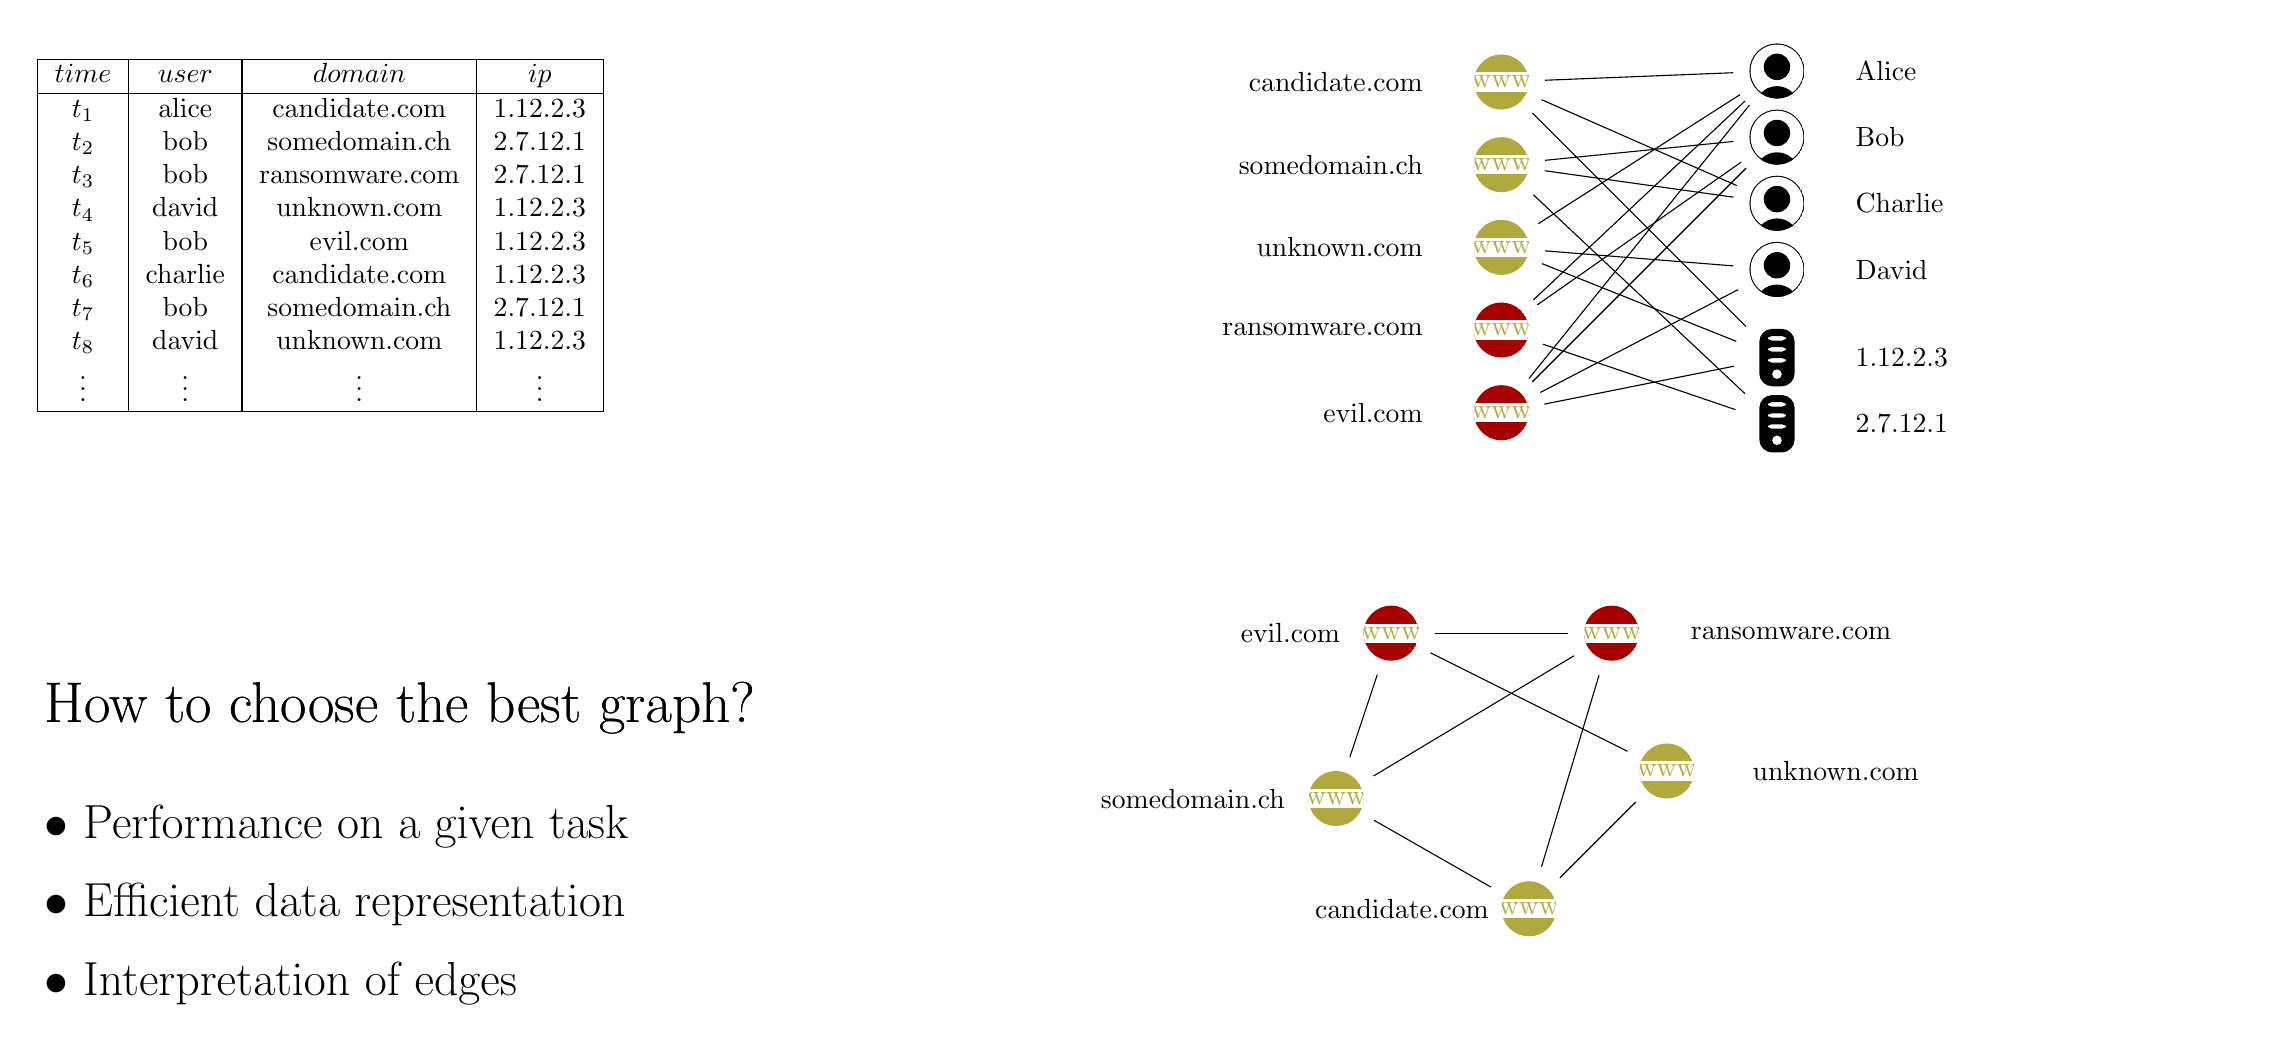
\begin{tikzpicture}

\node at (-15, 4) (x)
{
\begin{tabular}{|c|c|c|c|}
\hline
$\bm{time}$ & $\bm{user}$ & $\bm{domain}$ & $\bm{ip}$ \\
\hline
$t_1$&alice& candidate.com& 1.12.2.3\\
$t_2$&bob& somedomain.ch& 2.7.12.1\\
$t_3$&bob& ransomware.com& 2.7.12.1\\
$t_4$&david& unknown.com & 1.12.2.3\\
$t_5$&bob& evil.com & 1.12.2.3 \\
$t_6$&charlie& candidate.com & 1.12.2.3 \\
$t_7$&bob & somedomain.ch& 2.7.12.1 \\
$t_8$&david& unknown.com & 1.12.2.3\\
\vdots &\vdots &\vdots &\vdots \\
\hline
\end{tabular}
};

%{
%$\left\{\begin{array}{c}
%alice, candidate.com, 1.12.2.3\\
%bob, somedomain.ch, 2.7.12.1\\
%bob, ransomware.com, 2.7.12.1\\
%david, unknown.com , 1.12.2.3\\
%bob, evil.com , 1.12.2.3 \\
%charlie, candidate.com , 1.12.2.3 \\
%bob, somedomain.ch, 2.7.12.1 \\
%\dots
%\end{array}\right\}$};
%}
\begin{scope}[scale=0.7, yshift=4.5cm]   
  \malwwwline{-2}{evil.com}{D1};
  \malwwwline{-0.5}{ransomware.com}{D2};
  \wwwline{4}{candidate.com}{D5};
  \ipline{-1}{1.12.2.3}{i1}
  \userline{4.2}{Alice};
  \draw (Alice) -- (D1);
  \draw (Alice) -- (D2);
  \draw (i1) -- (D1);
  \draw (Alice) -- (D5);
  \draw (i1) -- (D5);
  \wwwline{1}{unknown.com}{D3};
  \wwwline{2.5}{somedomain.ch}{D4};
  \ipline{-2.2}{2.7.12.1}{i2}
  \userline{0.6}{David};
  \userline{1.8}{Charlie};
  \userline{3}{Bob};
  \draw (Alice) -- (D3);
  \draw (Bob) -- (D1);
  \draw (Bob) -- (D2);
  \draw (Bob) -- (D1);
  \draw (David) -- (D1);
  \draw (i2) -- (D2);
  \draw (Bob) -- (D4);
  \draw (David) -- (D3);
  \draw (Charlie) -- (D4);
  \draw (Charlie) -- (D5);
  \draw (i1) -- (D3);
  \draw (i2) -- (D4);

\end{scope}


\begin{scope}[scale=0.7, yshift=-4.5cm]  
\node[circle, minimum size=1.1cm] (d1) at (-2, 3) {};
\malwww{-2}{3}	\node[text width=50mm, align=right] at (-6.5, 3) {evil.com};

\node[circle, minimum size=1.1cm] (d2) at (2, 3) {};
\malwww{2}{3}	\node[text width=50mm, align=right] at (3.5, 3) {ransomware.com};

\node[circle, minimum size=1.1cm] (d3) at (-3, 0) {};
\www{-3}{0}	\node[text width=50mm, align=right] at (-7.5, 0) {somedomain.ch};

\node[circle, minimum size=1.1cm] (d4) at (3, 0.5) {};
\www{3}{0.5}	\node[text width=50mm, align=right] at (4, 0.5) {unknown.com};

\node[circle, minimum size=1.1cm] (d5) at (0.5, -2) {};
\www{0.5}{-2}	\node[text width=50mm, align=right] at (-3.8, -2) {candidate.com};

\draw (d1) -- (d2);
\draw (d1) -- (d3);
\draw (d1) -- (d4);
\draw (d2) -- (d3);
\draw (d2) -- (d5);
\draw (d3) -- (d5);
\draw (d4) -- (d5);

\end{scope}

\uncover<2>{
\node[font=\huge, text width=110mm, align=left] at (-13, -2) {
\alert{How to choose the best graph?}
};
}


\uncover<3->{
    \node[font=\huge, text width=110mm, align=left] at (-13, -2) {
How to choose the best graph?
};
    \node [font=\LARGE, text width=110mm, align=left] (top)    at (-13,-3.5) {$\bullet$ Performance on a given task};
    \node [font=\LARGE, text width=110mm, align=left] (middle) at (-13,-4.5)  {$\bullet$ Efficient data representation};
    \node [font=\LARGE, text width=110mm, align=left] (bottom) at (-13,-5.5)  {$\bullet$ Interpretation of edges};
}

\end{tikzpicture}
